\documentclass{article}

\usepackage[final]{neurips_2022}
\usepackage[utf8]{inputenc} % allow utf-8 input
\usepackage[T1]{fontenc}    % use 8-bit T1 fonts
\usepackage{hyperref}       % hyperlinks
\usepackage{url}            % simple URL typesetting
\usepackage{booktabs}       % professional-quality tables
\usepackage{amsfonts}       % blackboard math symbols
\usepackage{nicefrac}       % compact symbols for 1/2, etc.
\usepackage{microtype}      % microtypography
\usepackage{xcolor}         % colors
\usepackage{amsmath}
\usepackage{graphicx}
\usepackage{chemformula}

\title{CSCE 421: Final Project Write-Up}

\author{
    Huy Lai \\
    Texas A\&M University\\
    \texttt{lai.huy@tamu.edu} \\
}

\begin{document}


\maketitle

\begin{abstract}
  \begin{flushleft} 
   The objective of this model is to develop a predictive model for in-hospital mortality of patients receiving treatment.
   The dataset utilized in this study consists of information on several thousand patients during their 48-hour stay, including physical characteristics such as weight and height, and clinical measures such as mean heart rate, mean respiration rate, and mean \ch{O2} saturation.
   The data was employed to train an \verb+XGBoostClassifier+ model, which utilizes Gradient Boosting to accurately forecast the mortality of patients during their hospital stay.
   The proposed model achieved an Area Under the Receiver Operating Characteristic Curve (AUC-ROC) score of 0.89, demonstrating robust performance.
   This paper aims to provide a detailed account of the model's implementation and its results.
  \end{flushleft} 
\end{abstract}



\section{Introduction}
\begin{flushleft} 

The project has an objective of addressing a common issue in the healthcare industry.
Predicting patient mortality can aid healthcare professionals in providing tailored care and also facilitate comprehension of the relationship between patient care and mortality.
The resolution of this issue can have advantageous implications for preventive care in hospitals globally.
The eICU dataset was used to train the model, and relevant metrics such as Coma score, pH readings, blood pressure and heart rate were extracted.
These metrics are essential in evaluating a patient's wellbeing.
The model was trained and used to predict patient mortality using an \verb+XGBoostClassifier+.
The model achieved an AUC-ROC score of 0.89, compared to the baseline score of 0.84.

\end{flushleft}
    
\section{Method}
\begin{flushleft} 
The data was processed initially to extract pertinent characteristics that were thought to be linked to the mortality of patients.
Various classification models were tested subsequently to determine the best option for our circumstance.
Upon selecting XGBoostClassifier, efforts were made to tune the parameters of the model to optimize its performance.
Further elaboration on this procedure is provided in the subsequent sections, which will facilitate the replication of our findings.
\end{flushleft}
    
\subsection{Data Pre-Processing}
\begin{flushleft} 
Each row within the dataset contains unique data pertaining to test scores or important patient details documented by the staff.
Given that each row is associated with a distinct patient and test, it was deemed appropriate to iterate through all patient IDs and create a new dataframe for each individual.
This facilitated the extraction of key characteristics like height, weight, and gender.
Moreover, we identified subsets of the dataframe where the tests were similar, enabling us to compute average test scores, such as the average pH level.
Our aim was to account for all tests since a comprehensive medical approach necessitates the consideration of numerous factors that contribute to overall wellness.
Features like the average coma score were included as they are indicative of poor prognosis.

\clearpage
\noindent
The features, along with a brief summary, are provided below.
This approach was undertaken to acquire the most valuable insights pertaining to the patients' hospital stay.

\begin{table}[!ht]
    \centering
    \begin{tabular}{|l|l|}
        \hline
        \textbf{Feature} &   \textbf{Summary} \\ \hline  
        \verb+num_rows+ & Number of rows in dataset for each patient, illustrated numbers of test, etc. \\ \hline
        \verb+offset+ & Length of the patient's stay. \\ \hline
        \verb+height+ & Height of the patient in centimeters. \\ \hline
        \verb+weight+ & Weight of the patient in kilograms. \\ \hline
        \verb+gender+ & Biological Sex of the patient. \\ \hline
        \verb+avg_ph+ & Average pH reading of the patients during their stay. \\ \hline
        \verb+avg_glucose+ & Average glucose test results during their stay. \\ \hline
        \verb+num_visits+ & Number of visits a patient has had prior to the current visit. \\ \hline
        \verb+num_coma_tests+ & Number of times staff took a coma test. \\ \hline
        \verb+coma_score_avg+ & Average Score resulting from the coma tests. \\ \hline
        \verb+heart_rate_avg+ & Average Heart Rate reading during a patient's stay in beats per minute. \\ \hline
        \verb+resp_rate_avg+ & Average Respiratory Rate reading score during a patient's stay. \\ \hline
        \verb+saturation_avg+ & Average \ch{O2} saturation reading during a patient's stay. \\ \hline
        \verb+bp_avg+ & Average blood pressure reading during a patient's stay. \\ \hline
    \end{tabular}
    \caption{Features of the Model}
\end{table}
\end{flushleft}

\subsection{Model Design}
\begin{flushleft}
Numerous models were tested, as described in the results section below.
Ultimately, the XGBoost Classification model was selected based on its exceptional efficacy and efficiency.
Extreme Gradient Boosting is leveraged by XGBoost to produce highly accurate predictions.
As this is a classification problem, we employed the XGBoostClassifier instead of the regression model.
\end{flushleft}

\subsection{Model Training}
\begin{flushleft} 
The model training began with the implementation of an automated feature selector, which evaluated all the features listed in the table above and discarded those that had minimal impact on the model's performance.
\verb+gender+ and \verb+num_visits+ were among the features that were dropped, following which the model was trained. 
\end{flushleft}

\clearpage
\subsection{Hyperparameter Training}
\begin{flushleft}  
Grid search was utilized to optimize the model's performance by tuning its parameters.
This enabled us to evaluate various parameter values and determine the optimal combination that would yield the best outcome.
After conducting research on different hyperparameters, we determined the following parameters to be the most suitable:
\begin{itemize}
    \item \verb+`booster'+
    \item \verb+`learningrate'+
    \item \verb+`maxdepth'+
    \item \verb+`nestimators'+
    \item \verb+`regalpha'+
    \item \verb+`reglambda'+
    \item \verb+`minchildweight'+
    \item \verb+`subsample'+
    \item \verb+`colsamplebytree'+
    \item \verb+`gamma'+
    \item \verb+`scaleposweight'+
    \item \verb+`maxdeltastep'+
\end{itemize} 
\end{flushleft}

\section{Results}
\begin{flushleft} 

As mentioned earlier, three models were tested to identify the most suitable one.
Logistic Regression, Random Forest, and XGBoost were evaluated.
The graph below illustrates the AUC-ROC scores for each model in comparison to the baseline submission.

\begin{figure}[!ht]
    \centering
    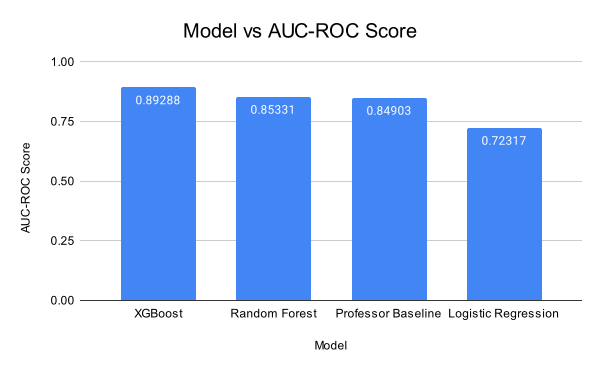
\includegraphics[width=0.9\textwidth]{scores.png}
    \caption{Various Models in comparison to their AUC-ROC Scores}
\end{figure}

\clearpage
The XGBoost model performed exceedingly well, achieving an AUC-ROC score of 0.893, as demonstrated above.
This score serves as a promising indicator that the model is proficient at accurately predicting patient mortality.
Additionally, the figure below illustrates the importance of each feature.

\begin{figure}[!ht]
    \centering
    \includegraphics[width=0.9\textwidth]{importance.png}
    \caption{Features and their importance to the model}
\end{figure}

The significance of this figure lies in its ability to showcase the influence of each feature on mortality classification.
Through a meticulous analysis of feature importance, healthcare practitioners can obtain a more comprehensive understanding of patient deaths.
In this instance, the heavily weighted feature is the coma score, implying that this metric demands closer scrutiny when determining patient health.
\end{flushleft}
    
\section{Conclusion}

\begin{flushleft} 

In conclusion, our model demonstrated remarkable performance, which can be attributed to the extensive experimentation conducted throughout the testing phase.
We evaluated diverse models, features, and implemented automated hyperparameter tuning.
This methodology facilitated the development of a proficient and reliable model, as analyzed in the results section.
To further enhance our outcomes, numerous additional techniques could be incorporated.
With additional time and resources, it would be possible to add more features by including some of the test types and their values that were left out.
Moreover, normalizing the data could boost the model's efficiency.
Nevertheless, our model performed substantially better than the baseline, leading us to believe that it is adept at predicting patient mortality.

\end{flushleft}
    
\end{document}
